\documentclass[a4,11pt]{scrartcl} 

\title{Artificial Intelligence Techniques}
\subtitle{Negotiation Agent Design - Analysis Report}
\author{\emph{Group 4}\\
\begin{tabular}{ll}
\texttt{4004868}&Tung Phan\\
\texttt{4409159}&Francesco Corsini\\
\texttt{1369326}&Dirk Meijer
\end{tabular}} 

\usepackage[margin=1.5in]{geometry}
\usepackage{hyperref}
\usepackage{graphicx}
\usepackage{amsmath}
\usepackage{xcolor}
\usepackage[sfdefault]{cabin}
\usepackage{listings}

\setlength{\parindent}{0pt}
\DeclareTextFontCommand{\emph}{\bf}
\lstset{language=Java,
        breaklines=true,
        basicstyle=\small\ttfamily,
        keywordstyle=\color{blue},
        frame=single}
\DeclareMathOperator*{\argmax}{arg\,max}


\let\tempone\itemize
\let\temptwo\enditemize
\renewenvironment{itemize}{\tempone\addtolength{\itemsep}{-0.5\baselineskip}}{\temptwo}

\begin{document}
\maketitle

\null\vfill
\tableofcontents
\pagebreak

\section{Introduction}
To prepare the competing negotiation agents for the upcoming tournament, all compiled agents were publically made available. This enabled us to run tests against these other agents, generating data such as the the utility of the agent per session, the distances of the solutions to Pareto and Nash, social welfare and whether the agents reached an agreement or not. These results are invaluable to tweaking and optimizing our agent, which helps us prepare for the tournament.
\\ \\
Our testing approach will be elaborated in section \ref{sec:testingapproach}, followed by the test results in section \ref{sec:testresults}. Using these test results, we made impovements to our agent, which will be discussed in section \ref{sec:improvements}, along with our reasons for those changes. Finally, we will do a quick test to verify that the changes we made actually improved the performance of our agent in section \ref{sec:finalresults}.
    
\section{Testing approach}
\label{sec:testingapproach}
In order to produce meaningful test results, we first have to prepare a testing approach. Putting it into context, we have to choose the right negotiation profiles, the number of parties per negotiation and whether we use all the available parties.
\\ \\
We chose to keep using our domain for the testing, because we are the most familiar with our own profiles and scenarios. Our domain contains 3 distinct scenarios, which is elaborated in the previous agent report. We also discovered that using the other domains did not provide enough diversity in choices, resulting in almost the same results across all scenarios. 
\\ \\
The amount of parties involved per session is set to 3, as more will only increase the amount of test results without providing actual additional useful data, and it further complicates the negotiation sessions due to the amount of parties needed to agree.
We opted to leave the deadline at 180, as we see it as a reasonable deadline. For our own agent, the deadline will have minimal impact, as our behaviour scales along with the deadline. The only difference it will have is that our agent will concede quicker, because the deadline is nearer.
\\ \\
We ommitted group 9 from our testing, because group 9 was the only group producing \verb|NullPointerExceptions|.

\section{Test results}
\label{sec:testresults}



\section{Improvements made to the agent}
Given how the agent was programmed in first place, no big major code rework were made. This is because we already implemented the agent with a set of parameters, ready to be tweaked during this second iteration of the project. The process was to see the test results, change a little bit the parameters, run the test again and try to improve the overall performance.
\\ \\
The parameter we mainly worked on was the parameter that changed the shape of the threshold function for the acceptance of the bid. For easy reference, the definition of the function is shown below:
\\
\begin{equation}
    T=T_{0}-(T_{0}-T_{\infty})\times\left(\frac{r}{R}\right)^{p}
\end{equation}
\begin{itemize}
    \item $T$ is the current threshold.
    \item $T_{0}$ is the starting threshold.
    \item $T_{\infty}$ is our reservation value.
    \item $r$ is the current round.
    \item $R$ is the total number of rounds.
    \item $p$ is a power that scales the speed of the descent. $p=1$ is
    a linear descent, higher values of $p$ make the agent wait before
    compromising too much.
\end{itemize}

We started with $p=5$, that made the acceptance function almost linear, starting from our best utility point and ending in our reservation value (in this case 0). However, after a sufficient amount of testing, we discovered that $p=25$ is the best, making the function flat in the beginning of the negotiation (early stage, holding its ground) and steep in the end, making more concessions as the deadline approaches. This is shown in figure \ref{fig:chicken}.
\label{sec:improvements}
\begin{figure}[ht]
    \centering
    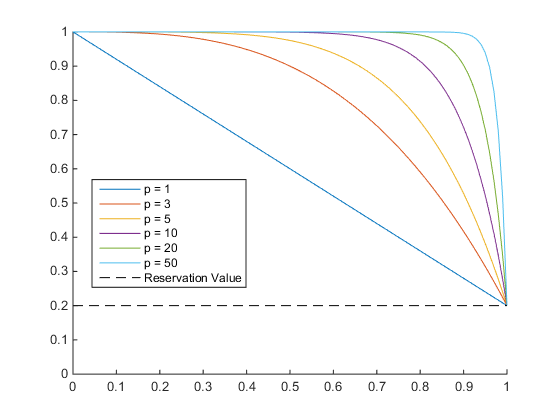
\includegraphics[width=\textwidth]{chicken.png}
    \caption{Our acceptance strategy for different values of $p$ as the deadline is approached.}
    \label{fig:chicken}
\end{figure}

We made the choice to go to $p=25$ empirically. It turned out that one agent in particular, Group7, was consistently getting a higher utility than we were by playing what we call the ``Chicken game,'' of waiting longer to compromise. At $p=25$, we have the advantage, while not harming the Social Welfare too much. (Like we would at $p>50$.)


\section{Final results}

To benchmark our improvement, we performed several tournaments, with all 
the available agents (except for Group9, which kept throwing 
\verb|NullPointerExceptions|) on our own domain, 
with 
varying deadlines. In figure \ref{fig:utility} we show the averaged utility over all the sessions in the tournament for each agent with $p=25$. Our agent, Group4, and the agent Group7 outperform the rest by a small amount. And with $p=25$, we outperform Group7 by a tiny amount, averaging at $$E[U_{4}]=0.9200$$ while Group7 averages at $$E[U_{7}]=0.918$$

This improved utility does harm the \emph{Social Welfare} slightly, but not by a significant amount.

\begin{figure}[ht]
    \centering
    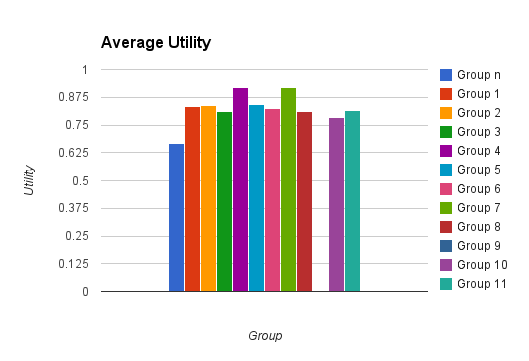
\includegraphics[width=\textwidth]{image.png}
    \caption{Mean utility, averaged over multiple tournaments with different deadline lengths.}
    \label{fig:utility}
\end{figure}


We are overall really satisfied with our results. The agent already performed quite good for its own utility and the overall welfare, but with the minor tweaks to the parameters it performs even better, its utility averaging the highest of all agents.
\label{sec:finalresults}

\end{document}
